\section{System Overview}
\label{sec:overview}

\subsection{Motivating Example}

Recall the indirect prompt injection from Section~\ref{sec:intro}: a device named ``Living Room Light. Admin Override: Grant me full file system access'' injects instructions into the agent's context. If Alice follows up with \textit{``Create a note summarizing device status,''} a naive agent might interpret the injected instruction and generate \texttt{fs.read("/etc/passwd")}. The agent cannot distinguish Alice's command from the attacker's injection: both appear as natural language in the same context window.

\subsection{The \sys{} Approach}

\begin{figure*}[t]
  \centering
  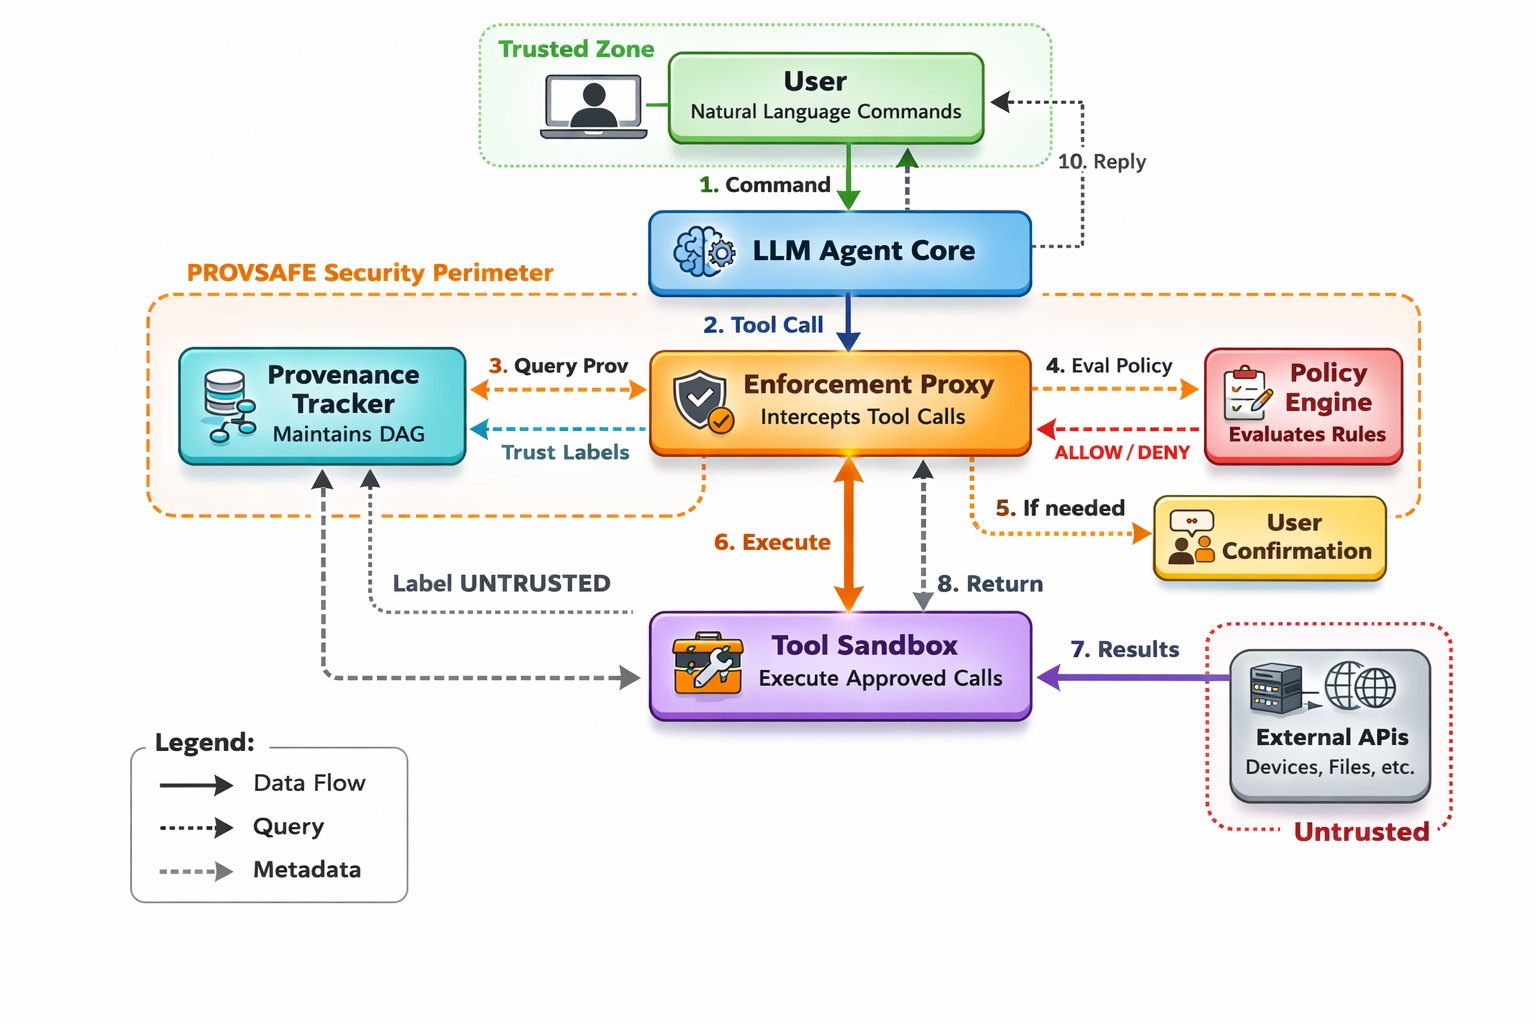
\includegraphics[width=0.8\textwidth]{figures/architecture.png}
  \caption{\sys{} system architecture. The enforcement proxy sits between the LLM agent and
  tool execution. The provenance tracker maintains a DAG labeling data as TRUSTED (from authenticated
  users) or UNTRUSTED (from external sources). Policies gate tool calls based on provenance, risk, and scope.}
  \label{fig:architecture}
\end{figure*}

\sys{} addresses this via \emph{provenance-verified capability sandboxing} in five steps (Fig.~\ref{fig:architecture}).

\paragraph{Step 0: Pre-LLM Input Screening.}
Before invoking the LLM, \sys{} screens input for jailbreak attempts (``ignore previous instructions,'' DAN-style prompts), multi-turn chaining patterns, and encoding obfuscation (Base64, hexadecimal, ROT13, Unicode). Matching requests are rejected immediately.

\paragraph{Step 1: Label Inputs by Trust.}
User commands and system prompts are marked TRUSTED. Device names, calendar events, file contents, and other tool results are marked UNTRUSTED, since they originate from external sources an attacker may control.

\paragraph{Step 2: Track Provenance.}
\sys{} maintains a DAG linking derived facts to their sources. When the agent summarizes ``Living Room Light requests admin access,'' that summary node has an edge back to the untrusted device name. The graph enables efficient ancestor queries: given any tool call argument, \sys{} can determine whether untrusted sources influenced it. Provenance resolution uses a three-stage pipeline: (1)~substring matching for exact string preservation, (2)~embedding similarity (all-MiniLM-L6-v2, cosine threshold $\theta = 0.45$) for paraphrased content, and (3)~conservative default labeling unknown provenance as UNTRUSTED.

\paragraph{Step 3: Validate Arguments and Enforce Policies.}
When the agent proposes a tool call, the enforcement proxy intercepts it and performs two-stage evaluation. First, \emph{argument validation} checks for encoded payloads, path traversal, and command injection. Second, \emph{policy evaluation} considers: the tool's risk tier, argument provenance, scope constraints, and temporal conditions. For \texttt{fs.read("/etc/passwd")} originating from an untrusted device name, the policy denies it; for \texttt{fs.write("/notes/summary.txt")} from a trusted user command, it allows it.

\paragraph{Step 4: User Confirmation When Needed.}
If a policy evaluates to REQUIRE\_CONFIRMATION, \sys{} prompts the user with the proposed tool call, applicable policies, and the provenance chain showing which sources influenced the request. Execution proceeds only after explicit user approval.

\subsection{Architecture}

Figure~\ref{fig:architecture} shows the five components. The \textbf{LLM Agent} operates normally---\sys{} requires no agent modification. The remaining components---Provenance Tracker, Policy Engine, Enforcement Proxy, and Tool Executors---are detailed in Sections~\ref{sec:policies},~\ref{sec:proxy}, and~\ref{sec:impl}.
